\section{Gabriela Żmuda}

\subsection{Twierdzenie sinusów}

\begin{figure}[htbp]
    \centering
    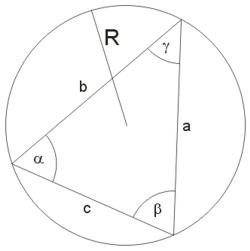
\includegraphics[width=0.3\textwidth]{pictures/sinus.jpg} 
    \caption{\label{fig:frog}Twierdzenie sinusów}
\end{figure}

Wzór na twierdzenie sinusów: \[a \sin \alpha = b \sin \beta = c \sin \gamma = 2 * R\]

Przykładowe wartości:

\begin{table}[htbp]
\centering
\begin{tabular}{||c c c c||} 
 \hline
 a & b & c & R \\ [0.5ex] 
 \hline\hline
 1 & 3 & 3 & 4 \\ 
 \hline
 5 & 8 & 7 & 9 \\
 \hline
 9 & 6 & 11 & 12 \\
 \hline
\end{tabular}
\label{tab:2}
\caption{Wymiary trojkatow}
\end{table}


\subsection{Zastosowanie}
Jak zastosować tewierdzenie sinusów:
\begin{enumerate}
    \item Sprawdź, jakie dane masz - sprawdź rysunek \ref{fig:frog}
    \item Sprawdź, jakich danych szukasz - sprawdź tabelkę \ref{tab:2}
    \item Użyj odpowiednio wzoru
    \item Dokonaj obliczeń
    \begin{enumerate}
        \item Jeśli się nie pomyliłeś, wypisz wynik
        \item Jeśli siś pomyliłeś, popraw błąd
    \end{enumerate}
\end{enumerate}

Uwagi:
\begin{itemize}
    \item Twierdzenie sinusów jest bardzo przydatne
    \item Warto je stosować
\end{itemize}

\subsection{Akapity}

Matematyka nas otacza, pomaga zrozumieć i opisać świat oraz wykonywać codzienne czynności. Jest to nauka złożona i nadrzędna wobec wielu innych dziedzin, ale kieruje się \textbf{logiką}. W matematyce wszystko jest ze sobą ściśle połączone i z siebie wynika, a to, wbrew pozorom, przysparza właśnie tak wiele trudności!

Matematyka jest \underline{praktyczną} dziedziną nauki, która w głównej mierze polega na rozwiązywaniu problemów. W tym celu trzeba mieć wiedzę, ale przede wszystkim – umieć ją wykorzystać w praktyce: dostrzegać pewne zależności i łączyć je w całości, analizować, szukać, myśleć, próbować, testować i sprawdzać. Wszystko to sprowadza się do tego, aby matematykę \textit{zrozumieć}. 